%% \documentclass{report}
%% 
%% \usepackage{fancyhdr}
\usepackage{fourier-orns}
\usepackage{hyperref}%% To refrence links / jumps
\usepackage{chngcntr} %% For some extra counters numberings
\usepackage[a4paper, right = 0.5in, left = 0.5in,top = 1in , bottom = 1in]{geometry}
\usepackage{etoolbox} %% Provides like a language for advanced customization
\usepackage{datetime} %% For dates of course
\usepackage{lastpage} %% provides pages numbers
\usepackage[sc]{titlesec} %% modify titles
\usepackage{enumerate}
\usepackage{cancel}
\usepackage{tikzsymbols}
\usepackage[dvipsnames]{xcolor}
\usepackage{import}
\usepackage{pdfpages} %% include other pdfs
\usepackage{transparent} %% Transparency
\usepackage{xcolor}  %% Colors
\usepackage[many]{tcolorbox}
\usepackage[framemethod=TikZ]{mdframed}
\usepackage{amsmath,amsfonts,amsthm,amssymb,mathtools}
\usepackage{tikz}
\usepackage{bookmark}
\usepackage{graphicx}
\usepackage{mathpazo}

\usepackage{fontawesome5}

\linespread{1.5}


\titleformat{\chapter}[display]   
{\fontfamily{ppl}\selectfont\huge\color{YellowOrange!80!orange}} % Font style and size 
{\raggedleft\color{purple}\fontsize{70}{0pt}\selectfont\thechapter}   
{-1.5cm}    			                          % Space between the chapter number and title
{
	\begin{tikzpicture}[overlay]
		\node[anchor = west,yshift = 0.2cm,xshift = -1cm] {\fontsize{90}{20} $\int_{}^{} $};
		\node[yshift = 4cm, xshift = 17cm]   {\includegraphics[width = 4cm]{preview0}};
	\end{tikzpicture}
\hspace{1cm}\Huge\raggedright\MakeUppercase}

\titleformat{\section}[block]
{
\fontfamily{ppl}\selectfont\huge\color{YellowOrange!80!orange}
}
{
\color{purple}\fontsize{20}{0pt}\selectfont\thesection 
}
{0cm}
{
	\begin{tikzpicture}[overlay]
		\node[anchor = west,yshift = 0.2cm,xshift = -0.4cm, circle = 1pt] {};
	\end{tikzpicture}
}

\titlespacing*{\section}{0pt}{0.7cm}{1.5cm}


\newcommand{\divider}
{
	\begin{center}
	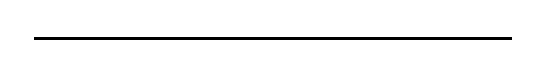
\begin{tikzpicture}
		\draw[thick, black] (0.25*\textwidth, 0) -- (0.75*\textwidth, 0);
		\node[rotate = 360 - 90, xshift = -0.6pt, yshift = 1pt] at (0.25*\textwidth,0){\decotwo};
		\node[rotate = 90, xshift = -0.6pt, yshift = 1pt] at (0.75*\textwidth,0){\decotwo};
	\end{tikzpicture}
	\end{center}
}

\pagestyle{fancy}

\newcommand{\lecday}[1][]
{
    \def\datee{#1}
    \fancyhead[L]{\datee}
}



\newcommand{\signature}
{
	\begin{tikzpicture}[remember picture,overlay]
		\node[fill = YellowOrange!20!white] at ([yshift = 1cm, xshift = -3cm]current page.south east) {\fontsize{10pt}{0pt}{\itshape Kara.$\mathcal{A}$}};
	\end{tikzpicture}
}

\AddToHook{shipout/background}{
  \begin{tikzpicture}[remember picture, overlay]
	  \node[] at ([yshift = 1.5cm,xshift = \textwidth /2 + 0.9cm]current page.south west) {\includegraphics[width = 0.5cm]{preview3}};
	  \node[] at ([yshift = 1.5cm,xshift = - \textwidth /2 - 0.9cm]current page.south east) {\includegraphics[width = 0.5cm]{preview4}};
  \end{tikzpicture}
}



\newtcolorbox[auto counter, number within = section]{remark}[1][]
{
       		title = Remark #1,
		enhanced,
		boxrule = 0pt,
		colback = white,
		breakable,
		arc = 4pt,
		colbacktitle = cyan,
		colback = cyan!5!white,
		segmentation style =
		{
			solid,cyan,thick,
		},
		attach boxed title to top left =
		{
			xshift = 0cm,
		},
		boxed title style =
		{
			boxrule = 0pt,
			sharp corners,
			drop fuzzy shadow = {cyan},
		},
		drop fuzzy shadow = {cyan!80!black},
}

\newtcolorbox[auto counter, number within = section]{theorem}[1][]
{                                      
		title = Theorem \thetcbcounter : #1,
		enhanced, 
		boxrule = 0pt,
		colback = white,
		breakable,
		arc = 4pt,
		colbacktitle = purple,
		colback = purple!5!white,
		segmentation style = 
		{
			solid, purple,thick,
		},
		attach boxed title to top left = 
		{
			xshift = 0cm, 
		},
		boxed title style = 
		{
			boxrule = 0pt,
			sharp corners,
			drop fuzzy shadow = {purple},
		},
		drop fuzzy shadow = {purple!80!black},
}

\newtcolorbox[auto counter, number within = section]{definition}[1][]
{                                      
		title = Definition \thetcbcounter : #1,
		enhanced, 
		boxrule = 0pt,
		colback = white,
		arc = 4pt,
		breakable,
		colbacktitle = YellowOrange!80!black,
		segmentation style = 
		{
			solid, YellowOrange,thick,
		},
		attach boxed title to top left = 
		{
			xshift = 0cm, 
		},
		colback = YellowOrange!5!white,
		boxed title style = 
		{
			boxrule = 0pt,
			sharp corners,
			drop fuzzy shadow = {YellowOrange!80!orange},
		},
		drop fuzzy shadow = {YellowOrange!80!black},
}

\newtcolorbox[auto counter, number within = section]{corollary}[1][]
{                                      
		title = corollary \thetcbcounter : #1,
		enhanced, 
		boxrule = 0pt,
		colback = white,
		arc = 4pt,
		breakable,
		colbacktitle = YellowOrange!80!black,
		segmentation style = 
		{
			solid, YellowOrange,thick,
		},
		attach boxed title to top left = 
		{
			xshift = 0cm, 
		},
		colback = YellowOrange!5!white,
		boxed title style = 
		{
			boxrule = 0pt,
			sharp corners,
			drop fuzzy shadow = {YellowOrange!80!orange},
		},
		drop fuzzy shadow = {YellowOrange!80!black},
}


\newtcolorbox{example}[1][]
{                                      
		title = Example,
		enhanced, 
		boxrule = 0pt,
		colback = white,
		arc = 4pt,
		segmentation style = 
		{
			solid, SpringGreen,thick,
		},
		breakable,
		colback = SpringGreen!5!white,
		colbacktitle = SpringGreen!80!black,
		attach boxed title to top left = 
		{
			xshift = 0cm, 
		},
		boxed title style = 
		{
			boxrule = 0pt,
			sharp corners,
			drop fuzzy shadow = {SpringGreen!80!orange},
		},
		drop fuzzy shadow = {SpringGreen!80!black},
}


\newcommand{\integral}[4]{\int\limits_{#1}^{#2} #4 d#3}
\newcommand{\limit}[3]{\lim\limits_{#1 \rightarrow #2} #3}
\newcommand{\strone}[2]{\left[ \begin{gathered}#1\\ #2\end{gathered} \right] }
\newcommand{\strtwo}[2]{\left\{ \begin{gathered}#1\\ #2\end{gathered} \right\} }
\newcommand{\strthree}[2]{\left\lfloor \begin{gathered}#1\\ #2\end{gathered} \right\rfloor }


\newcommand{\startbf}[1]{\text{\bfseries{#1}}}
\newcommand{\sett}[1]{\left\{ #1 \right\}}
\newcommand{\thesis}[1]{\left( #1 \right)}
\newcommand{\brkt}[1]{\left[ #1 \right]}
\newcommand{\floor}[1]{\left\lfloor #1 \right\rfloor}


\DeclareMathOperator{\img}{im} % Image
\DeclareMathOperator{\Img}{Im} % Image
\DeclareMathOperator{\coker}{coker} % Cokernel
\DeclareMathOperator{\Coker}{Coker} % Cokernel
\DeclareMathOperator{\Ker}{Ker} % Kernel
\DeclareMathOperator{\rank}{rank}
\DeclareMathOperator{\Spec}{Spec} % spectrum
\DeclareMathOperator{\Tr}{Tr} % trace
\DeclareMathOperator{\pr}{pr} % projection
\DeclareMathOperator{\ext}{ext} % extension
\DeclareMathOperator{\pred}{pred} % predecessor
\DeclareMathOperator{\dom}{dom} % domain
\DeclareMathOperator{\ran}{ran} % range
\DeclareMathOperator{\Hom}{Hom} % homomorphism
\DeclareMathOperator{\Mor}{Mor} % morphisms
\DeclareMathOperator{\End}{End} % endomorphism


\newcommand{\lm}{\ensuremath{\lambda}}
\newcommand{\eps}{\ensuremath{\epsilon}}
\newcommand{\veps}{\ensuremath{\varepsilon}}
\newcommand{\al}{\ensuremath{\alpha}}
\newcommand{\bb}{\ensuremath{\beta}}
\newcommand{\cc}{\ensuremath{\gamma}}
\newcommand{\dd}{\ensuremath{\delta}}
\newcommand{\DD}{\ensuremath{\Delta}}
\newcommand{\ff}{\ensuremath{\phi}}
\newcommand{\FF}{\ensuremath{\varphi}}

\newcommand{\RR}{\mathbb{R}}
\newcommand{\RO}{\mathcal{R}}
\newcommand{\EE}{\mathbb{E}}
\newcommand{\CC}{\mathbb{C}}
\newcommand{\RW}{\mathbb{R}^2}
\newcommand{\RT}{\mathbb{R}^3}
\newcommand{\RN}{\mathbb{R}^n}
\newcommand{\DS}{\mathcal{D}}

\newcommand{\KK}{\mathbb{K}}
\newcommand{\KW}{\mathbb{K}^2}
\newcommand{\KT}{\mathbb{K}^3}
\newcommand{\KN}{\mathbb{K}^n}

\newcommand{\NN}{\mathbb{N}}

\newcommand{\PS}{\mathcal{P}}
\newcommand{\AS}{\mathcal{E}}
\newcommand{\FS}{\mathcal{F}}
\newcommand{\LS}{\mathcal{L}}
\newcommand{\MS}{\mathcal{M}}

















%% 
\lecday[2025-04-15]

% \begin{document}

\divider
\textbf{Remainder} : \it(Separable spaces)\normalfont
A toplogical space is said to be separable if it 
contains a countable dense subset.
\divider
\begin{example}
$\RR$  equipped with its usual toplogy is separable
since $Q \subset \RR  $ is countable dense subset of
$\RR$, is a countable dense subset of 
$\RR$. More generally, $\RR ^n  $  
is seperable for all $n \in  \NN $  
(consider the subset $Q^{n} $ of $\RR ^n  $)
\end{example}
\divider
\textbf{
Generalization
}
Every finite dimensional N.V.S (Over $\RR$ or $\CC$  ) 
is separable, since, 
\[
E  \simeq  \KK^n  \simeq  \RR ^n  \simeq  \CC ^n 
\]
\divider
\begin{center}
	\textbf{An important exmaple}
\end{center}
\begin{theorem}[The weirstrass approximation theorem]
	Let $a,b \in \RR  $  with $a < b $, 
	then for every real valued continuous function on 
	$[a,b]  $, 
	there exist a real polynomial sequence $(P_{n}) _{n \in \NN} $  
	which uniformally converges to $f $ on $[a,b]$, in other 
	words, for every $ \veps  > 0 $, there exist a real polynomial
	 $P $ such that 
	 \[
	  \left| f(x) - p(x)  \right| <  \veps  
	  \quad  \left(  \forall  x \in  [a,b]  \right) 
	 \]
	 If $[a,b] = [0,1]$, we can take 
	 \[
	 P_{n}(x)  = 
	 \sum_{k = 0 }^{n}  
	 f(k/n) \binom{n}{k} x^{k}(1-x) ^{n-k}  
	 \]
	 The Bernestein polynomials associated to $f$ 
\end{theorem}
\it Consequence : \normalfont 
let $a,b \in  \RR  $, with $a < b$,
then N.V.S $(\mathcal{C} ^{0}([a,b], \RR , \| . \| _{\infty }))  $, 
is separable. Indeed, the subset of polynomail functions
with rational coefficients on $[a,b]  $ is countable and 
desne in $\left( \mathcal{C} ^{0}([a,b], \RR ), 
\| . \|_{\infty } \right) $  
\begin{definition}[]
Let $E $  be a N.V.S over $\KK=\RR  $  or $\CC $ 
\begin{enumerate}
\item A subset $S $ of $E $ is said to be total if 
	its span (i.e., the set of finite linear 
	combinations of elements of $E $ ) is dense.
\item A Hamel basis of $E $ is linearly independent 
	subset of $E $ which spans $E $ 
	(The concept already known in Linear Algebra-Algebra2)
It follows from Zorn's lemma that every vector space has 
a Hamel basis and that two Hamel bases of a same vector space
are necessarily equinumerous.
\item A schauder basis of $E $ is a sequence 
	$(l_{n}) _{n \in \NN} $  of $E $ such that 
	for each vector $x \in E $, there exists 
	a unique sequence $(\lm_{n}) _{n \in \NN} $  
	of scalars such that 
	\[
	x = \sum_{n=0}^{\infty}  \lm_{n} l_{n}
	\]
	that is, 
	\[
	\| x- \sum_{n=1}^{N} l_{n} \lm_{n} \| \rightarrow 0 
	\quad 0 \text{ as } N \rightarrow  \infty 
	\]
\end{enumerate}
\end{definition}
\begin{center}
	\textbf{Remark : }
\end{center}
\begin{enumerate}
\item Its easy to show that if a N.V.S $E $ has a Schauder basis
	then its separable (Exercise)
\item A Hamel basis (if its finite or countable) of a N.V.S 
	is always Schauder basis (obvious) but the converse is 
	false (see below!)
\item In a finite dimensional N.V.S the concept of Hamel basis and 
	Schauder basis coincides
\end{enumerate}
\begin{example}
\begin{enumerate}
\item (In relation with Fourier series let $p > 1 $, 
	It's show showed that the trigonometric, 
	\[
	1, \cos{(x) }, \sin{(x) }, \hdots   
	\]
	is a Schauder basis of the $\RR$-N.V.S $ L^{p}([0, 2\pi]) $, 
	\[
		L^{p}([0, 2\pi])  = 
		\left\{ f : [0, 2\pi] \rightarrow  \RR 
		\text{ s.t. } 
	\int_{0}^{2\pi} \left| f(x) \right|^{p} d(\mu (x) )  
	< \infty 
\right\} 
	\]
	with the norm $\| . \|_{p} $)
\item   Let $C_{0} $  denote the 
	$\RR  $-vector space of real sequences
	which converge to $0$ and let 
	\[
	\begin{array}{cccc}
	      \| . \| _{\infty } : &  
				   C_0& \longrightarrow & 
				   [0,\infty ]\\
	
	           &  x=(x_{n}) _{n \in \NN}  & \longmapsto     & 
		\| x \| _{\infty } := 
		\sup_{n \in  \NN} \left| x_{n} \right|\\ 
	\end{array}
	\]
\end{enumerate}
It's obvious that $\| . \| _{\infty } $  
is a norm on $C_0 $ (In fact $C_0 $ is a normed subspace of 
$(l^{\infty }, \| . \| _{\infty })  $), where,
\[
	l^{\infty } = 
	\left\{ \text{ the real bounded sequences }  \right\}
\]
for all $n \in  \NN $, let,
\[
l^{(n) } = (l_{i}^{(n) })  _{i \in  \NN}
\]
be the real sequence of $C_0 $ defined by, 
\[
l_{i}^{(n) } := 
\left\{ 
	1 
	\\
	0
\right\}
\begin{gathered}  
i = n \\  
0 \text{ else } 
\end{gathered} = 
(0, 0, \hdots , 0, 0, \ddots ) 
\in  C_0
\]
Its clear that $(e^{(n) })_{n \in \NN}  $  is linearly independent 
and is not a Hamel basis of $C_0$. Because 
\[
	\left\langle e^{(n) }, n \in \NN \right\rangle  = 
	C_{00} \neq C_0 
\]
where 
\[
C_{00} = 
\left\{ \text{ real sequences $(u_{N}) _{n \in \NN} $, for 
$u_{n}=  0 $ for $n $  sufficiently large }  \right\}
\]
$C_{00} \neq  C_0 $  
since we have for example 
$(\frac{1}{n}) _{n \in  \NN} \in C_0 $, but 
$(\frac{1}{n})_{n \in \NN} \notin  C_{00}$. 

Next, for any $x = (x_{n}) _{n \in \NN}  \in  C_0$, 
we have for $n \in \NN $,
\begin{align*}
	\| x - \sum_{n=1}^{N}  x_{n}e^{(n) } \| _{\infty } &=
	\| (x_1, x_2, \hdots ) - 
	(x_1, \hdots , x_{N}, 0, \hdots ) \|_{\infty }    \\
	&=  \| (0, \hdots , 0, x_{N+1}, \hdots )  \| _{\infty } \\
	&= \sup_{n \geq N+1} \left| x_{n} \right|    
\end{align*}
hence,
\begin{align*}
	\lim_{n \to \infty } 
	\| x - \sum_{n=1}^{N} x_{n}e^{(n) } \|  &= \lim_{n  \geq N+1}  
\sup_{}  \left| x_{n} \right| \\
						&=
						\overline{
						\lim_{n \to \infty} } 
						\left| x_{n} \right| \\ &= \lim_{n \to \infty } 
	\left| x_{n} \right| = 0
\end{align*}
This implies that the sequence 
$\left( \sum_{n=1}^{N} x_{n}e^{(n) } \right)_{n \in \NN} $   
of $C_0 $  is convergent to $x$. 

Equivalently, the series $\sum_{n=0}^{\infty}  x_{n}e^{(n) } $  
of $E $ is convergent to $x $, i.e. 
\[
x = \sum_{n=0}^{\infty}  
x_{n}e^{(n) } \quad \text{(in $C_0 $ )} 
\]
Let us show the uniqueness of a such representation of 
$x \in  C_0 $. Suppose that $x \in  C_0 $  is representable
as 
\[
x = \sum_{n=0}^{\infty}  \al_{n} e^{(n) } = 
\sum_{n=0}^{\infty}  \bb_{n} e^{(n) } \quad 
\left( \al_{n}, \bb _n \in  \RR, \forall n \in  \NN\right)
\]
we have for $n \in \NN $, 
\begin{align*}
\| \sum_{i=1}^{N} \al_{i} e^{(i) } - \sum_{i=1}^{N} \bb_{i} e^{(i) }\|   \\
&= \| \sum_{i=1}^{N} \left( \al_{i} - \bb_{i} \right)e^{i} \|  = 
\max_{ 1 \leq i \leq N} 
\left| \al_{i} - \bb_{i} \right|
\end{align*}                     
So for all $n, N \in \NN $, with $n \leq N $, we have, 
\[
\left| \al_{n} - \bb_{n} \right| \leq 
\max _{1 \leq i \leq N} 
\left| \al_{i} - b_{i} \right| =
\| \sum_{i=1}^{N} \al_{i} e^{(i)} - \sum_{i=1}^{N} \bb_{i} e^{(i) } \|  _{\infty }
\text{ By taking } N \rightarrow \infty 
\]
we get that, 
$\left| \al_{n} - \bb_{n} \right|  \leq  0 $, 
thus we have that,
\[
	\al_{n} = \bb_{n} \quad \quad \left( \forall n \in \NN \right)
\]
Thus, the representation of $x$, 
$\sum_{n=1}^{\infty } x_{n} e^{(n) } $ is unique. 

Consequently, $(e^{(n) })_{n \in \NN}  $  is a Schauder basis
of $C_0$ 
\end{example}
\divider
\chapter{Fundamental Theorems on banach spaces : }
\begin{itemize}
	\item The open mapping theorem.
	\item The closed graph theorem.
	\item The Banach-SteinHauns Theorem
	\item The Hahn-Banach 
\end{itemize}
\section{The open mapping theorem}
\textbf{Reminders : } 
A mapping $f $ from a toplogical space $X $ into a toplogical
space $Y $ is said to be an open mapping. if the image by $f $
of every open subset of $X $ is an open subset of $Y $ 
\begin{theorem}[(The open mapping theorem-Schaunder]
	Let $f $ be a continious linear mapping from 
	a Banach space $E $ to a Banach space $F $. Then
	the two following properties are equivalent,
	\begin{enumerate}[i]
	\item  $f $ is surjective
	\item $f $ is an open mapping 
	\end{enumerate}
\end{theorem}
\begin{proof}
\begin{center}
	$(ii)  \implies  (i) $  
\end{center}
We argue by contradiction. Suppose that $f $ is an open mapping
that $f $ is not surjective $(\text{ i.e. } . f(E)  \neq  F)  $, 
so $f(E) $, is a proper subspace of $F $, implying (see
the tutorial worksheet number $1 $ ), that 
\[
	int(f(E) )  = \emptyset 
\]
On the other hand, 
since $f $ is an open mapping and $E $ is open
in $E $ then $f(E)  $  is open in $F $, thus 
$int ( f(E))  = f(E)  $, Hence $f(E) = \emptyset   $, which is a contradiction.

\begin{center}
	$(i)  \implies  (ii)  $ 
\end{center}
we need preliminarry results.


\begin{theorem}[]
Let $E $ and $F $ be two N.V.S and 
$ f : E \longrightarrow F $ be a linear mapping 
then the two following properties are equivalent,
\begin{enumerate}[i]
\item  $f $ is an open mapping 
\item $\exists r > 0 $ such that 
	\[
	B_{F}(0_{F},r) \subset   f\left( B_{E}(0_{E},1)  \right) 
	\]
\end{enumerate}
\end{theorem}
\begin{proof}
	\begin{center}
		$(i)  \implies (ii)  $  
	\end{center}
	Suppose that $f $ is an open mapping. Since
	$B_{E}(0_{E}, 1)  $  is an open 
	subset of $E $, then 
	$f(B_{E}(0_{E},1) )  $  is an open subset of 
	$F $.
	So since,
	\[
	0_{F} = f(0_{E})  \in  f(B_{E}(0_{E},1) ) 
	\]
         then $f(B_{E}(0_{E},1) )  $  is a neighborhood of $0_{F} $, 
	 that is $\exists r > 0 $ such that 
	 \[
	 B_{F}(0_{F},r)   \subset f(B_{E}(0_{E},1) )  
	 \]
	 as required.
\end{proof}
\end{proof}
% \end{document}
